\documentclass[11pt,a4paper]{article}
\usepackage{gtu-el-yazisi}
\begin{document}
\notbilgi{İşaretler ve Sistemler}{Ders 3 -- Lineer zamanla değişmeyen (LZD / LTI) sistemler}{Isaret-ve-Sistemler-ders-3.pdf}
\renewcommand{\thempfootnote}{\alph{mpfootnote}} % kutu içi dipnotlar için (euler + \itshape uyumsuzluğu)

\section{Lineer Zamanla Değişmeyen (LZD) Sistemler:}
\sayfa{1}
Linear Time-Invariant (LTI) Systems

LTI sistemler detaylı olarak analiz edilebilirler
\begin{itemize}[label=--]
  \item Üst üste ekleme (superposition) özelliği
  \item Dürtü cevabı (impulse response) ile tüm karakteristik özellikleri belirlenebilir.
\end{itemize}

\textbf{\underline{Dürtü cevabı:}} Bir LTI sistemin dürtü cevabı $h(t)\,/\,h[n]$, sisteme birim dürtü işareti $\delta(t)\,/\,\delta[n]$ uygulandığında elde edilen çıkışıdır.
\begin{align*}
  x(t) = \delta(t) &\longrightarrow y(t) = h(t) \\
  x[n] = \delta[n] &\longrightarrow y[n] = h[n]
\end{align*}

$\Rightarrow$ Herhangi bir $x[n]\,/\,x(t)$ işareti, zamanda kaydırılmış birim dürtü işaretlerinin lineer kombinasyonu ile ifade edilebilir.
\[ x[n] = \sum_{k=-\infty}^{\infty} x[k]\,\delta[n-k] = \cdots + x[-1]\,\delta[n+1] + x[0]\,\delta[n] + x[1]\,\delta[n-1] + \cdots \]
\[ x(t) = \int_{-\infty}^{\infty} x(\tau)\,\delta(t-\tau)\,d\tau \]

\begin{ornek}[(Ex)]
\noindent
\begin{minipage}[c]{0.42\linewidth}
\centering
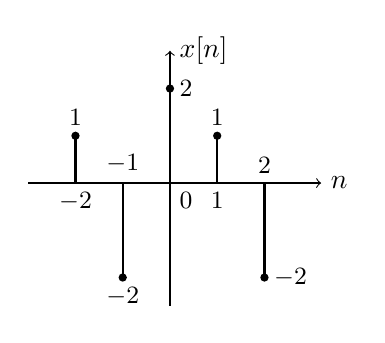
\begin{tikzpicture}[scale=0.6]
  \draw[->] (-3,0) -- (3.2,0) node[right] {$n$};
  \draw[->] (0,-2.6) -- (0,2.8) node[right] {$x[n]$};
  \foreach \x/\y in {-2/1,-1/-2,0/2,1/1,2/-2} { \draw[thick] (\x,0) -- (\x,\y); \fill (\x,\y) circle (2.5pt); }
  \node[above] at (-2,1) {\small $1$};
  \node[below] at (-1,-2) {\small $-2$};
  \node[right] at (0,2) {\small $2$};
  \node[above] at (1,1) {\small $1$};
  \node[right] at (2,-2) {\small $-2$};
  \node[below] at (-2,0) {\small $-2$};
  \node[above] at (-1,0) {\small $-1$};
  \node[below right] at (0,0) {\small $0$};
  \node[below] at (1,0) {\small $1$};
  \node[above] at (2,0) {\small $2$};
\end{tikzpicture}
\end{minipage}\hfill
\begin{minipage}[c]{0.55\linewidth}
Birim dürtü işareti cinsinden ifade ediniz.
\end{minipage}
\begin{align*}
  x[n] = \sum_{k=-2}^{2} x[k]\,\delta[n-k] &= x[-2]\,\delta[n+2] + x[-1]\,\delta[n+1] + x[0]\,\delta[n] \\
  &\quad + x[1]\,\delta[n-1] + x[2]\,\delta[n-2] \\
  &= \delta[n+2] - 2\,\delta[n+1] + 2\,\delta[n] + \delta[n-1] - 2\,\delta[n-2]
\end{align*}
\end{ornek}

\section{Ayrık zamanlı LTI sistemlerde konvolüsyon}
\sayfa{2}
\begin{center}
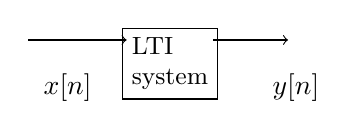
\begin{tikzpicture}
  \node[draw, align=left, font=\small] (S) at (0,0) {LTI\\system};
  \draw[->] (-1.8,0.3) -- (-0.55,0.3);
  \node at (-1.3,-0.3) {$x[n]$};
  \draw[->] (0.55,0.3) -- (1.5,0.3);
  \node at (1.6,-0.3) {$y[n]$};
\end{tikzpicture}
\end{center}
\begin{align*}
  x[n] = \delta[n] &\longrightarrow y[n] = h[n] \ : \ \text{Birim dürtü cevabı} \\
  x[n] = \delta[n-1] &\longrightarrow y[n] = h[n-1] \\
  x[n] = 3\,\delta[n+2] &\longrightarrow y[n] = 3\,h[n+2] \\
  x[n] = \sum_{k=-\infty}^{\infty} x[k]\,\delta[n-k] &\longrightarrow y[n] = \sum_{k=-\infty}^{\infty} x[k]\,h[n-k] \ : \ \text{Ayrık zamanlı konvolüsyon}
\end{align*}
\[ x[n] \longrightarrow \overset{\text{LTI}}{\boxed{h[n]}} \longrightarrow y[n] = x[n] \ast h[n] = \sum_{k=-\infty}^{\infty} x[k]\,h[n-k] = \sum_{k=-\infty}^{\infty} h[k]\,x[n-k] \]

\begin{ornek}[(Ex)]
\noindent
\begin{minipage}[c]{0.36\linewidth}
\centering
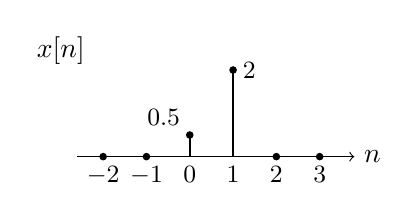
\begin{tikzpicture}[scale=0.55]
  \draw[->] (-2.6,0) -- (3.8,0) node[right] {$n$};
  \node[above left] at (-2.2,1.9) {$x[n]$};
  \foreach \x in {-2,-1,2,3} { \fill (\x,0) circle (2.5pt); }
  \foreach \x in {-2,...,3} { \node[below] at (\x,0) {\small $\x$}; }
  \draw[thick] (0,0) -- (0,0.5); \fill (0,0.5) circle (2.5pt); \node[above left] at (0,0.5) {\small $0.5$};
  \draw[thick] (1,0) -- (1,2); \fill (1,2) circle (2.5pt); \node[right] at (1,2) {\small $2$};
\end{tikzpicture}
\end{minipage}\hfill
\begin{minipage}[c]{0.36\linewidth}
\centering
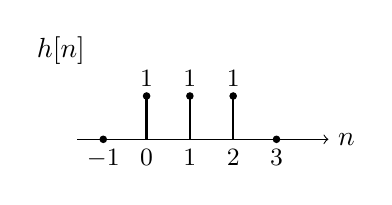
\begin{tikzpicture}[scale=0.55]
  \draw[->] (-1.6,0) -- (4.2,0) node[right] {$n$};
  \node[above left] at (-1.2,1.5) {$h[n]$};
  \foreach \x in {-1,3} { \fill (\x,0) circle (2.5pt); }
  \foreach \x in {-1,...,3} { \node[below] at (\x,0) {\small $\x$}; }
  \foreach \x in {0,1,2} { \draw[thick] (\x,0) -- (\x,1); \fill (\x,1) circle (2.5pt); \node[above] at (\x,1) {\small $1$}; }
\end{tikzpicture}
\end{minipage}\hfill
\begin{minipage}[c]{0.2\linewidth}
$y[n] = ?$
\end{minipage}
\end{ornek}
\begin{cozum}
\[ y[n] = x[n] \ast h[n] = \sum_{k=-\infty}^{\infty} x[k]\,h[n-k] \underset{\substack{\uparrow\\ k\,\in\,(0,1)}}{=} x[0]\,h[n] + x[1]\,h[n-1] = \underbrace{\underset{\substack{\downarrow\\ n\,\in\,(0,1,2)}}{0.5\,h[n]} + \underset{\substack{\downarrow\\ n\,\in\,(1,2,3)}}{2\,h[n-1]}}_{n\,\in\,(0,1,2,3)} \]

\noindent
\begin{minipage}[c]{0.4\linewidth}
\centering
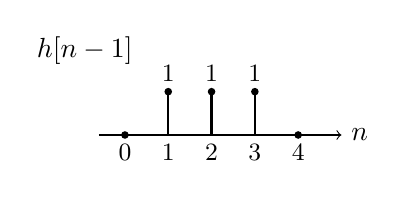
\begin{tikzpicture}[scale=0.55]
  \draw[->] (-0.6,0) -- (5,0) node[right] {$n$};
  \node[above left] at (0.4,1.4) {$h[n-1]$};
  \foreach \x in {0,4} { \fill (\x,0) circle (2.5pt); }
  \foreach \x in {0,...,4} { \node[below] at (\x,0) {\small $\x$}; }
  \foreach \x in {1,2,3} { \draw[thick] (\x,0) -- (\x,1); \fill (\x,1) circle (2.5pt); \node[above] at (\x,1) {\small $1$}; }
\end{tikzpicture}
\end{minipage}

\begin{align*}
  y[n] &= 0, \quad n \leq -1 \\
  y[0] &= 0.5\,h[0] + 2\,\underset{\swarrow 0}{h[-1]} = 0.5 \\
  y[1] &= 0.5\,h[1] + 2\,h[0] = 2.5 \\
  y[2] &= 0.5\,h[2] + 2\,h[1] = 2.5 \\
  y[3] &= 0.5\,\underset{\swarrow 0}{h[3]} + 2\,h[2] = 2 \\
  y[n] &= 0, \quad n \geq 4
\end{align*}

\begin{center}
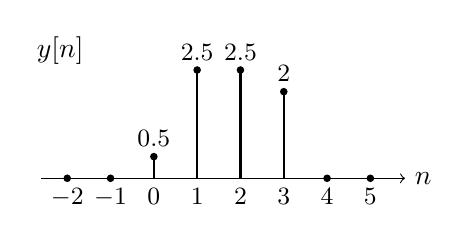
\begin{tikzpicture}[scale=0.55]
  \draw[->] (-2.6,0) -- (5.8,0) node[right] {$n$};
  \node[above left] at (-1.4,2.4) {$y[n]$};
  \foreach \x in {-2,-1,4,5} { \fill (\x,0) circle (2.5pt); }
  \foreach \x in {-2,...,5} { \node[below] at (\x,0) {\small $\x$}; }
  \foreach \x/\y/\l in {0/0.5/{0.5},1/2.5/{2.5},2/2.5/{2.5},3/2/{2}} { \draw[thick] (\x,0) -- (\x,\y); \fill (\x,\y) circle (2.5pt); \node[above] at (\x,\y) {\small $\l$}; }
\end{tikzpicture}
\end{center}
\end{cozum}

\begin{ornek}[(Ex)]
\sayfa{3}
$x[n] = \alpha^n u[n]$, \ $h[n] = u[n]$, \ $y[n] = ?$ \hfill \textcolor{linkrengi}{$0 < \alpha < 1$}
\end{ornek}
\begin{cozum}
\[ y[n] = \sum_{k=-\infty}^{\infty} x[k]\,h[n-k] = \sum_{k=-\infty}^{\infty} \alpha^k \underset{\substack{\downarrow\\ k \geq 0}}{u[k]}\ \underset{\substack{\downarrow\\ n-k \geq 0\\ n \geq k}}{u[n-k]} = \sum_{k=0}^{n} \alpha^k = \frac{1 - \alpha^{n+1}}{1 - \alpha}\,u[n] \]

\noindent
\begin{minipage}[c]{0.4\linewidth}
\centering
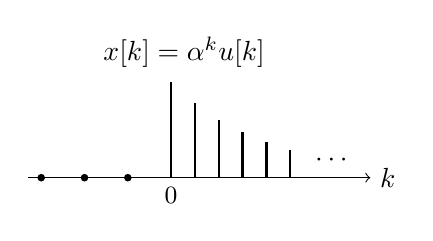
\begin{tikzpicture}[scale=0.55]
  \draw[->] (-3.3,0) -- (4.6,0) node[right] {$k$};
  \node at (0.3,2.9) {$x[k] = \alpha^k u[k]$};
  \foreach \x in {-3,-2,-1} { \fill (\x,0) circle (2.5pt); }
  \foreach \x in {0,...,5} { \draw[thick] ({0.55*\x},0) -- ({0.55*\x},{2.2*0.78^\x}); }
  \node at (3.7,0.4) {$\cdots$};
  \node[below] at (0,0) {\small $0$};
\end{tikzpicture}
\end{minipage}

\smallskip
\noindent
\begin{minipage}[c]{0.32\linewidth}
\centering
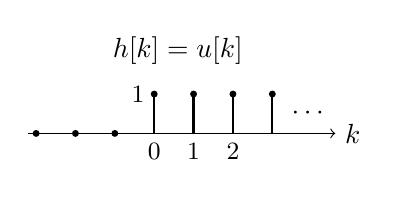
\begin{tikzpicture}[scale=0.5]
  \draw[->] (-3.2,0) -- (4.6,0) node[right] {$k$};
  \node at (0.6,2.1) {$h[k] = u[k]$};
  \foreach \x in {-3,-2,-1} { \fill (\x,0) circle (2.5pt); }
  \foreach \x in {0,1,2,3} { \draw[thick] (\x,0) -- (\x,1); \fill (\x,1) circle (2.5pt); }
  \node[left] at (0,1) {\small $1$};
  \node at (3.9,0.5) {$\cdots$};
  \foreach \x in {0,1,2} { \node[below] at (\x,0) {\small $\x$}; }
\end{tikzpicture}
\end{minipage}\hfill
\begin{minipage}[c]{0.32\linewidth}
\centering
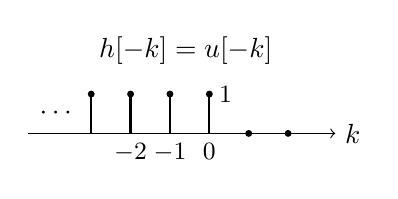
\begin{tikzpicture}[scale=0.5]
  \draw[->] (-4.6,0) -- (3.2,0) node[right] {$k$};
  \node at (-0.6,2.1) {$h[-k] = u[-k]$};
  \foreach \x in {1,2} { \fill (\x,0) circle (2.5pt); }
  \foreach \x in {-3,-2,-1,0} { \draw[thick] (\x,0) -- (\x,1); \fill (\x,1) circle (2.5pt); }
  \node[right] at (0,1) {\small $1$};
  \node at (-3.9,0.5) {$\cdots$};
  \foreach \x in {-2,-1,0} { \node[below] at (\x,0) {\small $\x$}; }
\end{tikzpicture}
\end{minipage}\hfill
\begin{minipage}[c]{0.32\linewidth}
\centering
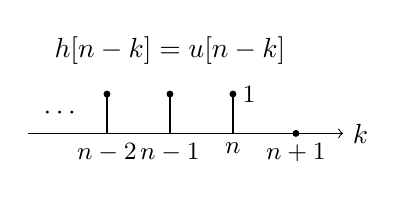
\begin{tikzpicture}[scale=0.5]
  \draw[->] (-5.2,0) -- (2.8,0) node[right] {$k$};
  \node at (-1.6,2.1) {$h[n-k] = u[n-k]$};
  \fill (1.6,0) circle (2.5pt);
  \foreach \x in {-3.2,-1.6,0} { \draw[thick] (\x,0) -- (\x,1); \fill (\x,1) circle (2.5pt); }
  \node[right] at (0,1) {\small $1$};
  \node at (-4.4,0.5) {$\cdots$};
  \node[below] at (-3.2,0) {\small $n-2$};
  \node[below] at (-1.6,0) {\small $n-1$};
  \node[below] at (0,0) {\small $n$};
  \node[below] at (1.6,0) {\small $n+1$};
\end{tikzpicture}
\end{minipage}
\end{cozum}

\begin{ornek}[(Ex)]
$x[n] = \begin{cases} 1, & \vurgu[turuncu]{$0 \leq n \leq 4$} \\ 0, & \text{dışında} \end{cases}$ \qquad
$h[n] = \begin{cases} \alpha^n, & 0 \leq n \leq 6 \\ 0, & \text{dışında} \end{cases}$ \qquad
$y[n] = ?$ \quad \textcolor{linkrengi}{$\alpha > 1$}
\end{ornek}
\begin{cozum}
\noindent
\begin{minipage}[c]{0.4\linewidth}
\centering
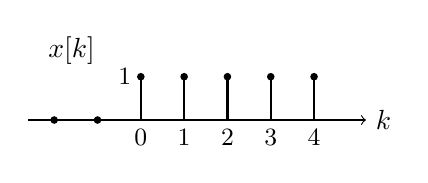
\begin{tikzpicture}[scale=0.55]
  \draw[->] (-2.6,0) -- (5.2,0) node[right] {$k$};
  \node at (-1.6,1.6) {$x[k]$};
  \foreach \x in {-2,-1} { \fill (\x,0) circle (2.5pt); }
  \foreach \x in {0,...,4} { \draw[thick] (\x,0) -- (\x,1); \fill (\x,1) circle (2.5pt); \node[below] at (\x,0) {\small $\x$}; }
  \node[left] at (0,1) {\small $1$};
\end{tikzpicture}
\end{minipage}\hfill
\begin{minipage}[c]{0.56\linewidth}
\centering
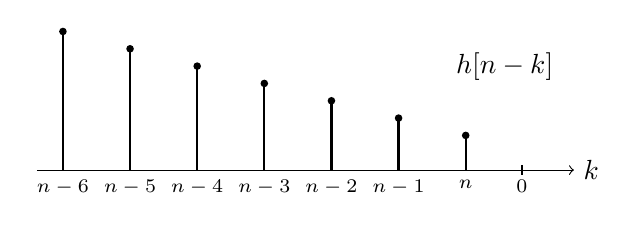
\begin{tikzpicture}[scale=0.55]
  \draw[->] (-0.6,0) -- (11.8,0) node[right] {$k$};
  \node at (10.2,2.4) {$h[n-k]$};
  \foreach \i in {0,...,6} { \draw[thick] ({1.55*\i},0) -- ({1.55*\i},{0.8+0.4*(6-\i)}); \fill ({1.55*\i},{0.8+0.4*(6-\i)}) circle (2.5pt); }
  \foreach \i/\l in {0/{n-6},1/{n-5},2/{n-4},3/{n-3},4/{n-2},5/{n-1},6/{n}} { \node[below] at ({1.55*\i},0) {\scriptsize $\l$}; }
  \draw (10.6,0.12) -- (10.6,-0.12); \node[below] at (10.6,0) {\scriptsize $0$};
\end{tikzpicture}
\end{minipage}

\begin{align*}
  n < 0 \qquad & y[n] = \sum_{k=-\infty}^{\infty} x[k]\,h[n-k] = 0 \\
  0 \leq n \leq 4 \qquad & y[n] = \sum_{k=0}^{n} x[k]\,h[n-k] = \sum_{k=0}^{n} \alpha^{n-k} \underset{\substack{\uparrow\\ n-k\,=\,r}}{=} \sum_{r=0}^{n} \alpha^r = \frac{1 - \alpha^{n+1}}{1 - \alpha} \\
  \left.\begin{aligned} n &> 4 \\ n-6 &\leq 0 \end{aligned}\right\}\ 4 < n \leq 6 \qquad & y[n] = \sum_{k=0}^{4} \alpha^{n-k} = \alpha^n \sum_{k=0}^{4} \alpha^{-k} = \alpha^n \cdot \frac{1 - (\alpha^{-1})^5}{1 - (\alpha^{-1})} = \frac{\alpha^{n-4} - \alpha^{n+1}}{1 - \alpha} \\
  \left.\begin{aligned} n &> 6 \\ n-6 &\leq 4 \end{aligned}\right\}\ 6 < n \leq 10 \qquad & y[n] = \sum_{k=n-6}^{4} \alpha^{n-k} \underset{\substack{\uparrow\\ r\,=\,k-n+6}}{=} \sum_{r=0}^{10-n} \alpha^{6-r} = \alpha^6 \sum_{r=0}^{10-n} \alpha^{-r} \\
  & \phantom{y[n]} = \alpha^6\,\frac{1 - \alpha^{n-11}}{1 - \alpha^{-1}} = \frac{\alpha^{n-4} - \alpha^7}{1 - \alpha} \\
  n - 6 > 4 \rightarrow n > 10 \qquad & y[n] = 0
\end{align*}

\[ y[n] = \begin{cases}
  0, & n < 0 \\[1mm]
  \dfrac{1 - \alpha^{n+1}}{1 - \alpha}, & 0 \leq n \leq 4 \\[3mm]
  \dfrac{\alpha^{n-4} - \alpha^{n+1}}{1 - \alpha}, & 4 < n \leq 6 \\[3mm]
  \dfrac{\alpha^{n-4} - \alpha^{7}}{1 - \alpha}, & 6 < n \leq 10 \\[2mm]
  0, & n > 10
\end{cases} \]
\end{cozum}

\section{Sürekli Zamanlı LTI Sistemlerde Konvolüsyon}
\sayfa{4}
\[ x(t) \longrightarrow \overset{\text{LTI}}{\boxed{h(t)}} \longrightarrow y(t) = x(t) \ast h(t) = \int_{-\infty}^{\infty} x(\tau)\,h(t-\tau)\,d\tau = \int_{-\infty}^{\infty} h(\tau)\,x(t-\tau)\,d\tau \]

\begin{ornek}[(Ex)]
$x(t) = e^{-at}u(t)$, \ $a > 0$, \quad $h(t) = u(t)$, \quad $y(t) = ?$
\end{ornek}
\begin{cozum}
\begin{center}
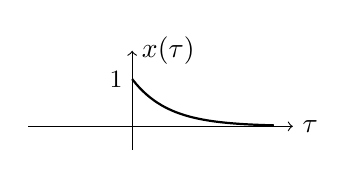
\begin{tikzpicture}[scale=0.6]
  \draw[->] (-2.2,0) -- (3.4,0) node[right] {$\tau$};
  \draw[->] (0,-0.5) -- (0,1.6) node[right] {$x(\tau)$};
  \draw[thick, domain=0:3, samples=40] plot (\x, {exp(-1.3*\x)});
  \node[left] at (0,1) {\small $1$};
\end{tikzpicture}
\end{center}
\noindent
\begin{minipage}[c]{0.32\linewidth}
\centering
\begin{tikzpicture}[scale=0.55]
  \draw[->] (-2.6,0) -- (3,0) node[right] {$\tau$};
  \draw[->] (0,0) -- (0,1.8) node[right] {$h(\tau)$};
  \draw[thick] (-2.4,0) -- (0,0); \draw[thick] (0,1) -- (2.6,1);
  \node[left] at (0,1) {\small $1$}; \node[below] at (0,0) {\small $0$};
\end{tikzpicture}
\end{minipage}\hfill
\begin{minipage}[c]{0.32\linewidth}
\centering
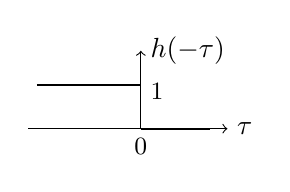
\begin{tikzpicture}[scale=0.55]
  \draw[->] (-2.6,0) -- (2,0) node[right] {$\tau$};
  \draw[->] (0,0) -- (0,1.8) node[right] {$h(-\tau)$};
  \draw[thick] (-2.4,1) -- (0,1); \draw[thick] (0,0) -- (1.6,0);
  \node[right] at (0,0.85) {\small $1$}; \node[below] at (0,0) {\small $0$};
\end{tikzpicture}
\end{minipage}\hfill
\begin{minipage}[c]{0.32\linewidth}
\centering
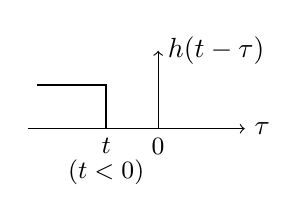
\begin{tikzpicture}[scale=0.55]
  \draw[->] (-3,0) -- (2,0) node[right] {$\tau$};
  \draw[->] (0,0) -- (0,1.8) node[right] {$h(t-\tau)$};
  \draw[thick] (-2.8,1) -- (-1.2,1) -- (-1.2,0);
  \node[below] at (-1.2,0) {\small $t$}; \node[below] at (0,0) {\small $0$};
  \node at (-1.2,-1) {\small $(t<0)$};
\end{tikzpicture}
\end{minipage}

\[ y(t) = x(t) \ast h(t) = \int_{-\infty}^{\infty} x(\tau)\,h(t-\tau)\,d\tau \]
\begin{align*}
  t < 0 \qquad & y(t) = 0 \\
  t \geq 0 \qquad & y(t) = \int_{0}^{t} e^{-a\tau}\,d\tau = \frac{e^{-a\tau}}{-a}\Bigg|_{0}^{t} = \frac{1}{a}\bigl(1 - e^{-at}\bigr)
\end{align*}
\[ y(t) = \frac{1}{a}\bigl(1 - e^{-at}\bigr)\,\vurgu[yesil]{$u(t)$} \]
\begin{center}
\begin{tikzpicture}[scale=0.6]
  \draw[->] (-0.5,0) -- (5,0) node[right] {$t$};
  \draw[->] (0,-0.3) -- (0,2.3) node[right] {$y(t)$};
  \draw[thick, domain=0:4.5, samples=50] plot (\x, {1.6*(1-exp(-1.1*\x))});
  \draw[dashed, kursunkalem] (0,1.6) -- (4.5,1.6);
  \node[left] at (0,1.6) {$\frac{1}{a}$};
\end{tikzpicture}
\end{center}
\end{cozum}

\begin{ornek}[(Ex)]
$x(t) = e^{2t}u(-t)$, \quad $h(t) = u(t-3)$, \quad $y(t) = ?$
\end{ornek}
\begin{cozum}
\begin{center}
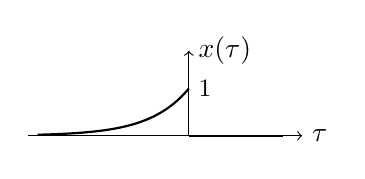
\begin{tikzpicture}[scale=0.6]
  \draw[->] (-3.4,0) -- (2.4,0) node[right] {$\tau$};
  \draw[->] (0,0) -- (0,1.8) node[right] {$x(\tau)$};
  \draw[thick, domain=-3.2:0, samples=40] plot (\x, {exp(1.2*\x)});
  \draw[thick] (0,0) -- (2,0);
  \node[right] at (0,1) {\small $1$};
\end{tikzpicture}
\end{center}
\noindent
\begin{minipage}[c]{0.32\linewidth}
\centering
\begin{tikzpicture}[scale=0.55]
  \draw[->] (-1.4,0) -- (4.2,0) node[right] {$\tau$};
  \draw[->] (0,0) -- (0,1.8) node[right] {$h(\tau)$};
  \draw[thick] (-1.2,0) -- (2,0) -- (2,1) -- (3.8,1);
  \draw[dashed, kursunkalem] (0,1) -- (2,1);
  \node[left] at (0,1) {\small $1$}; \node[below] at (2,0) {\small $3$};
\end{tikzpicture}
\end{minipage}\hfill
\begin{minipage}[c]{0.32\linewidth}
\centering
\begin{tikzpicture}[scale=0.55]
  \draw[->] (-4,0) -- (1.6,0) node[right] {$\tau$};
  \draw[->] (0,0) -- (0,1.8) node[right] {$h(-\tau)$};
  \draw[thick] (-3.8,1) -- (-2,1) -- (-2,0) -- (1.2,0);
  \draw[dashed, kursunkalem] (-2,1) -- (0,1);
  \node[right] at (0,1) {\small $1$}; \node[below] at (-2,0) {\small $-3$};
\end{tikzpicture}
\end{minipage}\hfill
\begin{minipage}[c]{0.32\linewidth}
\centering
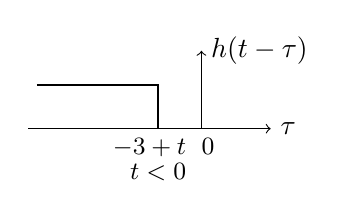
\begin{tikzpicture}[scale=0.55]
  \draw[->] (-4,0) -- (1.6,0) node[right] {$\tau$};
  \draw[->] (0,0) -- (0,1.8) node[right] {$h(t-\tau)$};
  \draw[thick] (-3.8,1) -- (-1,1) -- (-1,0);
  \node[below] at (-1.2,0) {\small $-3+t$}; \node[below] at (0.15,0) {\small $0$};
  \node at (-1,-1) {\small $t<0$};
\end{tikzpicture}
\end{minipage}

\sayfa{5}
\begin{align*}
  t - 3 \leq 0 \qquad & y(t) = \int_{-\infty}^{t-3} e^{2\tau}\,d\tau = \frac{1}{2}\,e^{2\tau}\Bigg|_{-\infty}^{t-3} = \frac{1}{2}\,e^{2(t-3)} \\
  t - 3 > 0 \qquad & y(t) = \int_{-\infty}^{0} e^{2\tau}\,d\tau = \frac{1}{2}
\end{align*}
\[ y(t) = \begin{cases} 0.5\,e^{2(t-3)}, & t \leq 3 \\ 0.5, & t > 3 \end{cases} \]
\end{cozum}

\begin{ornek}[(Ex)]
$x(t) = \begin{cases} 1, & 0 < t < T \\ 0, & \text{dışında} \end{cases}$, \qquad
$h(t) = \begin{cases} t, & 0 < t < 2T \\ 0, & \text{dışında} \end{cases}$, \qquad $y(t) = ?$
\end{ornek}
\begin{cozum}
\[ y(t) = x(t) \ast h(t) = \int_{-\infty}^{\infty} x(\tau)\,h(t-\tau)\,d\tau = \int_{-\infty}^{\infty} h(\tau)\,x(t-\tau)\,d\tau \]
\begin{center}
\begin{tikzpicture}[scale=0.6]
  \draw[->] (-1,0) -- (3.4,0) node[right] {$\tau$};
  \draw[->] (0,-0.3) -- (0,2.4) node[right] {$h(\tau)$};
  \draw[thick] (-1,0) -- (0,0) -- (2.4,1.8);
  \draw[dashed, kursunkalem] (2.4,1.8) -- (2.4,0);
  \node[below] at (2.4,0) {\small $2T$};
  \draw (-0.1,1.8) -- (0.1,1.8); \node[left] at (0,1.8) {\small $2T$};
\end{tikzpicture}
\end{center}
\noindent
\begin{minipage}[c]{0.32\linewidth}
\centering
\begin{tikzpicture}[scale=0.55]
  \draw[->] (-1.2,0) -- (3.4,0) node[right] {$\tau$};
  \draw[->] (0,0) -- (0,1.8) node[right] {$x(\tau)$};
  \draw[thick] (0,1) -- (1.8,1) -- (1.8,0);
  \node[left] at (0,1) {\small $1$}; \node[below] at (1.8,0) {\small $T$};
\end{tikzpicture}
\end{minipage}\hfill
\begin{minipage}[c]{0.32\linewidth}
\centering
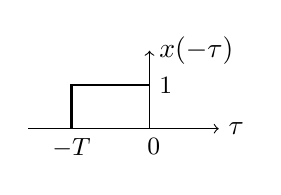
\begin{tikzpicture}[scale=0.55]
  \draw[->] (-2.8,0) -- (1.6,0) node[right] {$\tau$};
  \draw[->] (0,0) -- (0,1.8) node[right] {$x(-\tau)$};
  \draw[thick] (-1.8,0) -- (-1.8,1) -- (0,1);
  \node[right] at (0,1) {\small $1$}; \node[below] at (-1.8,0) {\small $-T$}; \node[below] at (0.1,0) {\small $0$};
\end{tikzpicture}
\end{minipage}\hfill
\begin{minipage}[c]{0.32\linewidth}
\centering
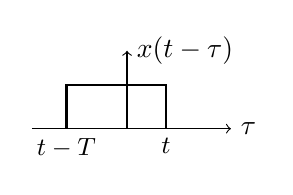
\begin{tikzpicture}[scale=0.55]
  \draw[->] (-2.2,0) -- (2.4,0) node[right] {$\tau$};
  \draw[->] (0,0) -- (0,1.8) node[right] {$x(t-\tau)$};
  \draw[thick] (-1.4,0) -- (-1.4,1) -- (0.9,1) -- (0.9,0);
  \node[below] at (-1.4,0) {\small $t-T$}; \node[below] at (0.9,0) {\small $t$};
\end{tikzpicture}
\end{minipage}

\begin{align*}
  t < 0 \qquad & y(t) = 0 \\
  0 < t < T \qquad & y(t) = \int_{0}^{t} \tau\,d\tau = \frac{\tau^2}{2}\Bigg|_{0}^{t} = t^2/2 && \longleftarrow \ \begin{aligned} &t > 0 \\[-1mm] &t - T < 0 \end{aligned} \\
  T < t < 2T \qquad & y(t) = \int_{t-T}^{T} \tau\,d\tau = \frac{\tau^2}{2}\Bigg|_{t-T}^{T} = \frac{T^2}{2} - \frac{(t-T)^2}{2} = tT - T^2/2 \quad \text{\footnotemark} && \longleftarrow \ \begin{aligned} &t < 2T \\[-1mm] &t - T > 0 \end{aligned} \\
  2T < t < 3T \qquad & y(t) = \int_{t-T}^{2T} \tau\,d\tau = \frac{\tau^2}{2}\Bigg|_{t-T}^{2T} = -\frac{t^2}{2} + Tt + \frac{3T^2}{2} && \longleftarrow \ \begin{aligned} &t > 2T \\[-1mm] &t - T < 2T \end{aligned} \\
  t > 3T \qquad & y(t) = 0
\end{align*}
\[ y(t) = \begin{cases}
  0, & t < 0 \\
  t^2/2, & 0 < t < T \\
  tT - T^2/2, & T < t < 2T \\
  -t^2/2 + Tt + 3T^2/2, & 2T < t < 3T \\
  0, & t > 3T
\end{cases} \]
\end{cozum}
\footnotetext{Claude notu: $T<t<2T$ satırında muhtemelen üst sınır $t$ olmalı: $\int_{t-T}^{t}\tau\,d\tau = \frac{t^2}{2} - \frac{(t-T)^2}{2} = tT - T^2/2$ (yazılan sonuç bununla uyumlu).}

\section{Konvolüsyon işleminin özellikleri}
\sayfa{6}
\subsection{1) Yer değiştirme (commutative) özelliği}
\begin{align*}
  y[n] &= x[n] \ast h[n] = \sum_{k=-\infty}^{\infty} x[k]\,h[n-k] = \sum_{k=-\infty}^{\infty} h[k]\,x[n-k] \\
  y(t) &= x(t) \ast h(t) = \int_{-\infty}^{\infty} x(\tau)\,h(t-\tau)\,d\tau = \int_{-\infty}^{\infty} h(\tau)\,x(t-\tau)\,d\tau
\end{align*}

\subsection{2) Dağılma (distributive) özelliği}
\begin{align*}
  x[n] \ast \bigl(h_1[n] + h_2[n]\bigr) &= x[n] \ast h_1[n] + x[n] \ast h_2[n] \\
  x(t) \ast \bigl[h_1(t) + h_2(t)\bigr] &= x(t) \ast h_1(t) + x(t) \ast h_2(t)
\end{align*}
\begin{center}
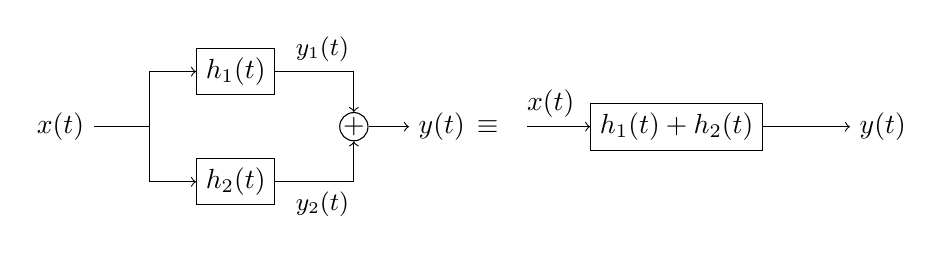
\begin{tikzpicture}
  \node[draw, minimum height=0.55cm] (A) at (1.4,0.7) {$h_1(t)$};
  \node[draw, minimum height=0.55cm] (B) at (1.4,-0.7) {$h_2(t)$};
  \node[draw, circle, inner sep=0pt, minimum size=0.32cm] (S) at (2.9,0) {$+$};
  \draw (-0.4,0) node[left] {$x(t)$} -- (0.3,0);
  \draw[->] (0.3,0) |- (A.west);
  \draw[->] (0.3,0) |- (B.west);
  \draw[->] (A.east) -| node[pos=0.3, above] {\small $y_1(t)$} (S.north);
  \draw[->] (B.east) -| node[pos=0.3, below] {\small $y_2(t)$} (S.south);
  \draw[->] (S.east) -- (3.6,0) node[right] {$y(t)$};
  \node at (4.6,0) {$\equiv$};
  \node[draw, minimum height=0.6cm] (C) at (7,0) {$h_1(t) + h_2(t)$};
  \draw[->] (5.1,0) node[right] {} -- (C.west); \node[above] at (5.4,0) {$x(t)$};
  \draw[->] (C.east) -- (9.2,0) node[right] {$y(t)$};
\end{tikzpicture}
\end{center}
\begin{center}
Dağılma özelliği $\equiv$ Paralel Bağlama \ (Only for LTI)
\end{center}

\subsection{3) Birleşme (associative) özelliği}
\begin{align*}
  x[n] \ast \bigl(h_1[n] \ast h_2[n]\bigr) &= \bigl(x[n] \ast h_1[n]\bigr) \ast h_2[n] = x[n] \ast h_1[n] \ast h_2[n] \\
  x(t) \ast \bigl[h_1(t) \ast h_2(t)\bigr] &= \bigl[x(t) \ast h_1(t)\bigr] \ast h_2(t) = x(t) \ast h_1(t) \ast h_2(t)
\end{align*}
\begin{center}
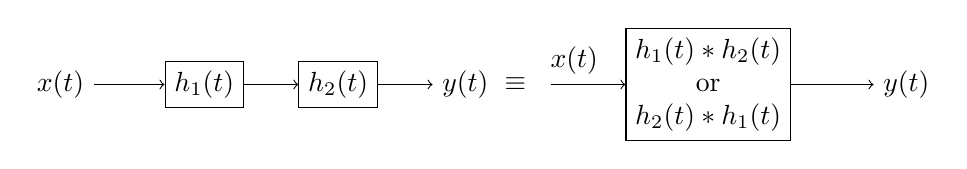
\begin{tikzpicture}
  \node[draw, minimum height=0.55cm] (A) at (0.8,0) {$h_1(t)$};
  \node[draw, minimum height=0.55cm] (B) at (2.5,0) {$h_2(t)$};
  \draw[->] (-0.6,0) node[left] {$x(t)$} -- (A.west);
  \draw[->] (A.east) -- (B.west);
  \draw[->] (B.east) -- (3.7,0) node[right] {$y(t)$};
  \node at (4.75,0) {$\equiv$};
  \node[draw, align=center] (C) at (7.2,0) {$h_1(t) \ast h_2(t)$\\ or\\ $h_2(t) \ast h_1(t)$};
  \draw[->] (5.2,0) -- (C.west); \node[above] at (5.5,0) {$x(t)$};
  \draw[->] (C.east) -- (9.3,0) node[right] {$y(t)$};
\end{tikzpicture}
\end{center}
\begin{center}
Birleşme özelliği $\equiv$ Seri Bağlama \ (Only for LTI)
\end{center}

\section{LTI sistemlerin özellikleri}
LTI sistemlerin özellikleri birim dürtü cevabı üzerinden belirlenebilir.

\subsection{1) Hafızaya sahip olan ve olmayan LTI sistemler}
(LTI systems with and without memory)

\noindent
\begin{minipage}[t]{0.5\linewidth}
Bellekli ve belleksiz LTI sistemler
\end{minipage}\hfill
\begin{minipage}[t]{0.47\linewidth}
\small Reminder: Bir sistemin herhangi bir zamandaki çıkışı, sadece o andaki girişlere bağlı ise belleksizdir.
\end{minipage}
\[ y[n] = x[n] \ast h[n] = \sum_{k=-\infty}^{\infty} x[k]\,h[n-k] = \sum_{k=-\infty}^{\infty} h[k]\,x[n-k] \]
\noindent
\begin{minipage}[c]{0.7\linewidth}
\begin{align*}
  \text{Belleksiz: } & h[n] = 0, \ n \neq 0 \\
  & h[n] = K\delta[n] \longrightarrow y[n] = x[n] \ast h[n] = K\,x[n] \ast \delta[n] = K\,x[n] \\
  \text{Reminder: } & x[n] \ast \delta[n] = \sum_{k=-\infty}^{\infty} x[k]\,\delta[n-k] = x[n]
\end{align*}
\end{minipage}\hfill
\begin{minipage}[c]{0.27\linewidth}
\fcolorbox{kirmizikalem}{kagitrengi}{\parbox{0.9\linewidth}{\color{turuncukalem}\small h[n]=1, n=0,1\\ =d[n]+d[n-1]\\[2mm] x[n]\\ y[n]=x[n]+x[n-1]}}
\end{minipage}

\begin{align*}
  & y(t) = x(t) \ast h(t) = \int_{-\infty}^{\infty} x(\tau)\,h(t-\tau)\,d\tau \\
  & h(t) = 0, \ t \neq 0 \\
  & h(t) = K\delta(t) \longrightarrow y(t) = K\,x(t) \\
  & \text{Reminder: } x(t) \ast \delta(t) = \int_{-\infty}^{\infty} x(\tau)\,\delta(t-\tau)\,d\tau = x(t)
\end{align*}

\subsection{2) Tersinir ve tersinir olmayan LTI sistemler:}
\sayfa{7}
Reminder: Bir sistem, tersi ile seri bağlandığında elde edilen çıktı ile girdi aynı ise sistem tersinirdir.
\begin{center}
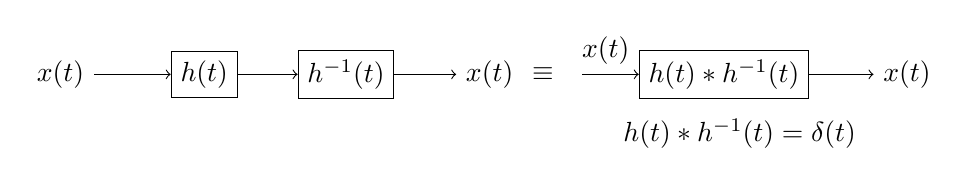
\begin{tikzpicture}
  \node[draw, minimum height=0.55cm] (A) at (0.8,0) {$h(t)$};
  \node[draw, minimum height=0.55cm] (B) at (2.6,0) {$h^{-1}(t)$};
  \draw[->] (-0.6,0) node[left] {$x(t)$} -- (A.west);
  \draw[->] (A.east) -- (B.west);
  \draw[->] (B.east) -- (4,0) node[right] {$x(t)$};
  \node at (5.1,0) {$\equiv$};
  \node[draw, minimum height=0.6cm] (C) at (7.4,0) {$h(t) \ast h^{-1}(t)$};
  \draw[->] (5.6,0) -- (C.west); \node[above] at (5.9,0) {$x(t)$};
  \draw[->] (C.east) -- (9.3,0) node[right] {$x(t)$};
  \node at (7.6,-0.75) {$h(t) \ast h^{-1}(t) = \delta(t)$};
\end{tikzpicture}
\end{center}
Tersinir: \ $h(t) \ast h^{-1}(t) = \delta(t)$

$\Rightarrow$ LTI bir sistemin tersi de LTI'dır.
\[ h[n] \ast h^{-1}[n] = \delta[n] \]

\begin{ornek}[(Ex)]
$y(t) = x(t-t_0)$ sistemi tersinir midir?
\end{ornek}
\begin{cozum}
\[ y(t) = x(t) \ast h(t) = x(t-t_0) \longleftarrow h(t) = \delta(t-t_0) \longrightarrow y(t) = x(t) \ast \delta(t-t_0) = \int_{-\infty}^{\infty} x(\tau)\,\delta(t-t_0-\tau)\,d\tau \]
\begin{align*}
  &= \int_{-\infty}^{\infty} x(t-t_0)\,\delta(t-t_0-\tau)\,d\tau \\
  &= x(t-t_0) \underbrace{\int_{-\infty}^{\infty} \delta(t-t_0-\tau)\,d\tau}_{1} = x(t-t_0)
\end{align*}
\begin{align*}
  & h(t) \ast h^{-1}(t) = \delta(t) \\
  & h^{-1}(t) = \delta(t+t_0) \\
  & \quad \delta(t-t_0) \ast \delta(t+t_0) = \delta(t) \qquad \text{Tersinirdir.}
\end{align*}
\end{cozum}

\begin{ornek}[(Ex)]
Birim dürtü cevabı $h[n] = u[n]$ olan LTI bir sistem tersinir midir?
\end{ornek}
\begin{cozum}
\begin{center}
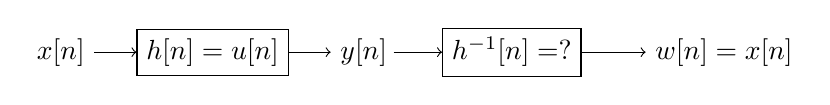
\begin{tikzpicture}
  \node[draw, minimum height=0.55cm] (A) at (0.9,0) {$h[n] = u[n]$};
  \node[draw, minimum height=0.55cm] (B) at (4.7,0) {$h^{-1}[n] = ?$};
  \draw[->] (-0.6,0) node[left] {$x[n]$} -- (A.west);
  \draw[->] (A.east) -- (2.4,0) node[right] {$y[n]$};
  \draw[->] (3.2,0) -- (B.west);
  \draw[->] (B.east) -- (6.4,0) node[right] {$w[n] = x[n]$};
\end{tikzpicture}
\end{center}
\begin{align*}
  y[n] &= x[n] \ast h[n] = \sum_{k=-\infty}^{\infty} x[k]\,u[n-k] = \sum_{k=-\infty}^{n} x[k] \\
  w[n] &= y[n] - y[n-1] = \sum_{k=-\infty}^{n} x[k] - \sum_{k=-\infty}^{n-1} x[k] \\
  &= \bigl(\cdots + x[n-1] + x[n]\bigr) - \bigl(\cdots + x[n-2] + x[n-1]\bigr) = x[n]
\end{align*}
$\hookrightarrow$ \ $h^{-1}[n] = \delta[n] - \delta[n-1]$
\begin{align*}
  & h[n] \ast h^{-1}[n] \overset{?}{=} \delta[n] \\
  & u[n] \ast \bigl(\delta[n] - \delta[n-1]\bigr) = u[n] \ast \delta[n] - u[n] \ast \delta[n-1] = u[n] - u[n-1] = \delta[n] \ \checkmark \quad \text{Tersinir.}
\end{align*}
\end{cozum}

\end{document}
